\pattern{Factory}
\begin{summary}
    The {\bf Factory} method pattern is a class-creation design pattern,
    meaning that its purpose is to deal with object creation.

    The factory method pattern creates a predefined interface for object
    creation within a parent class, while at the same time allowing for
    child classes to determine exactly what type of objects are created. This
    makes it so that object creation responsibility falls on the child classes,
    and the class that uses the new object can treat the process of object
    creation as a black-box. The class only needs to be concerned with
    providing the correct data and it can assume that the correct object will
    be instantiated and returned to them.

    This pattern proves to be very useful over time as it can significantly
    reduce maintenance costs.
\end{summary}

\subsubsection{Implementation}
The Factory pattern standarizes object creation through the use of inheritance
and subclasses to instantiate objects. It uses a ``factory method'' to create
objects, rather than the developer using the constructor of the objects
themselves. This allows for greater flexibility and dynamism when determining
what type of object to construct. This factory method is specified within an
interface in a parent class, whose behaviour is then implemented by child
classes. These child classes are then responsible for the actual instantiation
of the object, and can specify the type of the object. This pattern allows for
many different child classes that can all implement the factory method and
return different types.

\comparison{\begin{itemize}
        \item Readability: It provides a level of abstraction for object
            creation. Instead of a developer needing to fully understand
            what subclass they need and how to instantiate it, they can use the
            factory’s exposed method to generate an instance. 
            
        \item Low coupling: Allows for a separation of concerns between an
            object’s creation and usage. There is a level of abstraction that
            means the object instantiated can be determined at runtime. 
            The developer can request an object that will meet the abstract
            product’s requirements without knowing what subclass will be 
            created.

        \item Encapsulation: This pattern can help developers hide the
            implementation details of the subclass by only exposing an
            interface to the user. This leads to a decrease in coupling within
            the overall application. 
        \item Maintainability: The factory method pattern also improves
            the maintainability of the system. Developers only need to create a
            new subclass which implements the exposed common interface in order
            to create a new type without bother implementing the entire
            structure of the new class type.
    \end{itemize}

}{\begin{itemize}
        \item Efficiency: If it is not used within the correct scenarios. The
            additional layer of overhead that the pattern adds by requiring the
            creation of subclasses that are tasked with object creation can 
            become inefficient. With simple, low complexity classes that do not
            change, it is much easier to just instantiate objects within the
            parent class rather than delegate that works to child classes.

        \item Maintainability: If the pattern is overused to allow for dynamism
            within a system that does not need it, it will become overly
            complex. If every object is created through a factory method (thus
            creating new base classes, base products, and each concrete
            implementation) the code will be unnecessarily complex, difficult
            to follow, and hard to test. Thus this design pattern should only
            be used when its benefits clearly outweighs the added overhead.
    \end{itemize}
}% END comparison

\begin{nfps}
\item[Evolvability] All that is required to meet new requirements is to create
    another subclass of the object with the new functionality.
\item[Complexity] Components can be created and perceived as their parent
    class. The developer only has to work with the abstraction and not the
    specifics, thus decreasing the overall complexity of the system.
\item[Negative Efficiency] The added overhead of creating child
    classes can be quite expensive.
\item[Negative Complexity] The additional abstraction through the factory can
    negate any complexity benefits, and even make the code base more complex
    and difficult to understand.
\end{nfps}

\begin{center}
    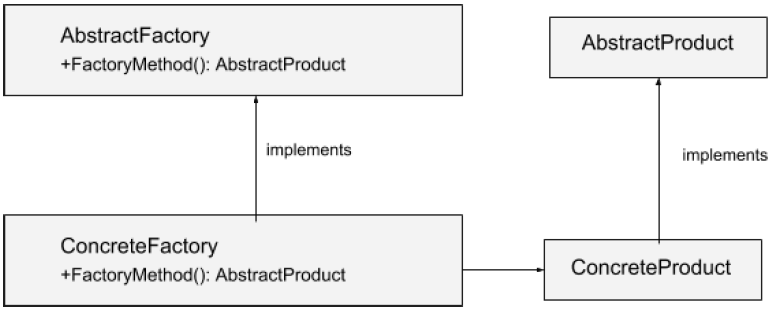
\includegraphics[width=0.8\textwidth]{./factory}
\end{center}
